\documentclass[9pt,twocolumn,twoside]{gsajnl_modified}
% Use the documentclass option 'lineno' to view line numbers

\usepackage[htt]{hyphenat}  % https://tex.stackexchange.com/a/543
\usepackage[export]{adjustbox}
\usepackage{xurl}
\usepackage{stfloats}
\usepackage{sidecap}

\renewcommand{\topfraction}{0.9}	% max fraction of floats at top
    \renewcommand{\bottomfraction}{0.8}	% max fraction of floats at bottom
    %   Parameters for TEXT pages (not float pages):
    \setcounter{topnumber}{2}
    \setcounter{bottomnumber}{2}
    \setcounter{totalnumber}{4}     % 2 may work better
    \setcounter{dbltopnumber}{2}    % for 2-column pages
    \renewcommand{\dbltopfraction}{0.9}	% fit big float above 2-col. text
    \renewcommand{\textfraction}{0.07}	% allow minimal text w. figs
    %   Parameters for FLOAT pages (not text pages):
    \renewcommand{\floatpagefraction}{0.7}	% require fuller float pages
	% N.B.: floatpagefraction MUST be less than topfraction !!
    \renewcommand{\dblfloatpagefraction}{0.7}	% require fuller float pages

\title{An antibody-escape calculator for mutations to the SARS-CoV-2 receptor-binding domain}

\author[*]{\Large Allison J. Greaney$^{1,2,3}$, Tyler N. Starr$^{1,4}$, Jesse D. Bloom$^{1,2,4}$}

\affil[1]{Basic Sciences and Computational Biology, Fred Hutchinson Cancer Center

} 
\affil[2]{Department of Genome Sciences, University of Washington

}
\affil[3]{Medical Scientist Training Program, University of Washington

}
\affil[4]{Howard Hughes Medical Institute

Seattle, WA, USA
}

\keywords{}

\runningtitle{} % For use in the footer 
\runningauthor{}

\begin{abstract}
A key goal of SARS-CoV-2 surveillance is to rapidly identify viral variants with mutations that reduce neutralization by polyclonal antibodies elicited by vaccination or infection.
Unfortunately, direct experimental characterization of new viral variants lags their sequence-based identification. 
Here we help address this challenge by providing an ``escape calculator'' that estimates the antigenic effects of arbitrary combinations of mutations to the virus's spike receptor-binding domain (RBD).
Specifically, the calculator aggregates deep mutational scanning data to visualize how mutations impact polyclonal antibody recognition.
It also scores how much each mutant is expected to escape RBD-targeted antibody neutralization.
These scores correlate with neutralization assays performed by multiple labs on a range of SARS-CoV-2 variants, and emphasize the ominous antigenic properties of the recently described Omicron variant.
An interactive version of the calculator is at \url{https://jbloomlab.github.io/SARS2_RBD_Ab_escape_maps/escape-calc/}, and we provide a Python module for batch processing.
\end{abstract}

\begin{document}

\maketitle
\thispagestyle{firststyle}
%\marginmark
\firstpagefootnote

\correspondingauthoraffiliation{}{*Corresponding author: \href{mailto:jbloom@fredhutch.org}{jbloom@fredhutch.org}}
\vspace{-33pt}% Only used for adjusting extra space in the left column of the first page

\lettrine[lines=2]{\color{color2}H}{}uman coronaviruses undergo rapid antigenic evolution that erodes antibody-based neutralization~\citep{eguia2021human,kistler2021evidence}.
This antigenic evolution is already apparent for SARS-CoV-2, as new viral variants with reduced antibody neutralization have already emerged only $\sim$2 years since the virus first started to spread in humans~\citep{?}.
A tremendous amount of experimental effort has been expended to characterize these SARS-CoV-2 variants in neutralization assays~\citep{?}.
Unfortunately, the rate at which new variants arise outstrips the speed with which these experiments can be performed.

A partial solution is to use deep mutational scanning to \emph{prospectively} characterize how viral mutations impact antibody binding or neutralization.
Deep mutational scanning can systematically the antigenic impacts of all possible amino-acid mutations in key regions of spike on specific antibodies~\citep{starr2021prospective,greaney2021complete} or sera~\citep{greaney2021comprehensive}.
However, SARS-CoV-2 variants of concern typically have multiple mutations in spike, and it is not feasible to characterize all combinations of mutations even via high-throughput approaches such as deep mutational scanning.

Here we take a step towards addressing this challenge by aggregating deep mutational scanning data across many antibodies to assess the impacts of combinations of mutations in the spike receptor-binding domain (RBD), which is the primary target of neutralizing antibodies to SARS-CoV-2~\citep{?}.
The resulting ``escape calculator'' enables both qualitative visualization and quantitative scoring of the antigenic impacts of arbitrary combinations of RBD mutations.
Importantly, the escape calculator is based on simple and intuitive transformations of direct experimental measurements, and does not involve complex black-box computational methods. 

\section{Results}

\subsection{Combining monoclonal antibody escape maps reveals correlated and independent viral antigenic mutations}
A deep mutational scanning experiment can measure how all single amino-acid mutations to the SARS-CoV-2 RBD affect binding by a monoclonal antibody.
This mutation-level information can be summarized for each RBD site, such as by taking the mean or sum of mutation-level effects at a site.
Here we will work with these site-level escape maps.

As a small example to illustrate the principle behind our approach, Figure~\ref{fig:mini_example}A shows previously reported measurements~\citep{starr2021prospective, starr2021complete} of how mutations to each RBD site affect binding by three monoclonal antibodies: LY-CoV016 (etesevimab), LY-CoV555 (bamlanivimab), and REGN10987 (imdevimab).
Each antibody targets a different one of the three main neutralizing epitopes on the RBD: LY-CoV016 targets the class 1 epitope, LY-CoV555 the class 2 epitope, and REGN10987 the class 3 epitope~\citep{barnes2020sars,greaney2021mapping}.
Because the antibodies have distinct epitopes, they are each escaped by largely distinct sets of mutations: LY-CoV016 is most strongly escaped by mutations at site K417, LY-CoV555 at site E484, and REGN10987 at sites K444 to G446 (Figure~\ref{fig:mini_example}A).

Now imagine a polyclonal antibody mix consisting of these three antibodies combined at equal potencies.
We can generate a site-level ``escape map'' for this hypothetical antibody mix simply by averaging the experimentally measured escape maps for the three individual antibodies, yielding the thick black line in Figure~\ref{fig:mini_example}A.
Because this polyclonal escape map is the average of the three monoclonal antibody escape maps, its largest peaks are at the sites of strongest escape for each of the individual antibodies: sites K417, E484, and K444 to G446.

Next imagine removing one antibody from the mix by mutating its epitope.
Figure~\ref{fig:mini_example}B shows the resulting escape map if LY-CoV555 is ablated, as would occur if site E484 was mutated.
The thick black line for the antibody mix no longer has peaks at E484 and other sites targeted by LY-CoV555, such as F490.
Therefore, in this hypothetical polyclonal antibody mix, escape at sites E484 and F490 is correlated since both are targeted by the same antibody.
However, the polyclonal mix's escape map at sites K417 and N460 is unaffected by mutations that escape LY-CoV555, since they are targeted by a different antibody, LY-CoV016.
But if we also ablate LY-CoV016 (such as by mutating site K417), then the peaks at K417 and N460 also disappear, and the most remaining peaks are at sites targeted by REGN10987, such as K444 to G446 (Figure~\ref{fig:mini_example}C).
Of course, if REGN10987 was also ablated such as by mutating site G446, then the polyclonal antibody mix would have no remaining activity.
(This and other scenarios can be explored using the interactive version of Figure~\ref{fig:mini_example} at \url{https://jbloomlab.github.io/SARS2_RBD_Ab_escape_maps/mini-example-escape-calc/}.)

\begin{SCfigure*}[0.3]
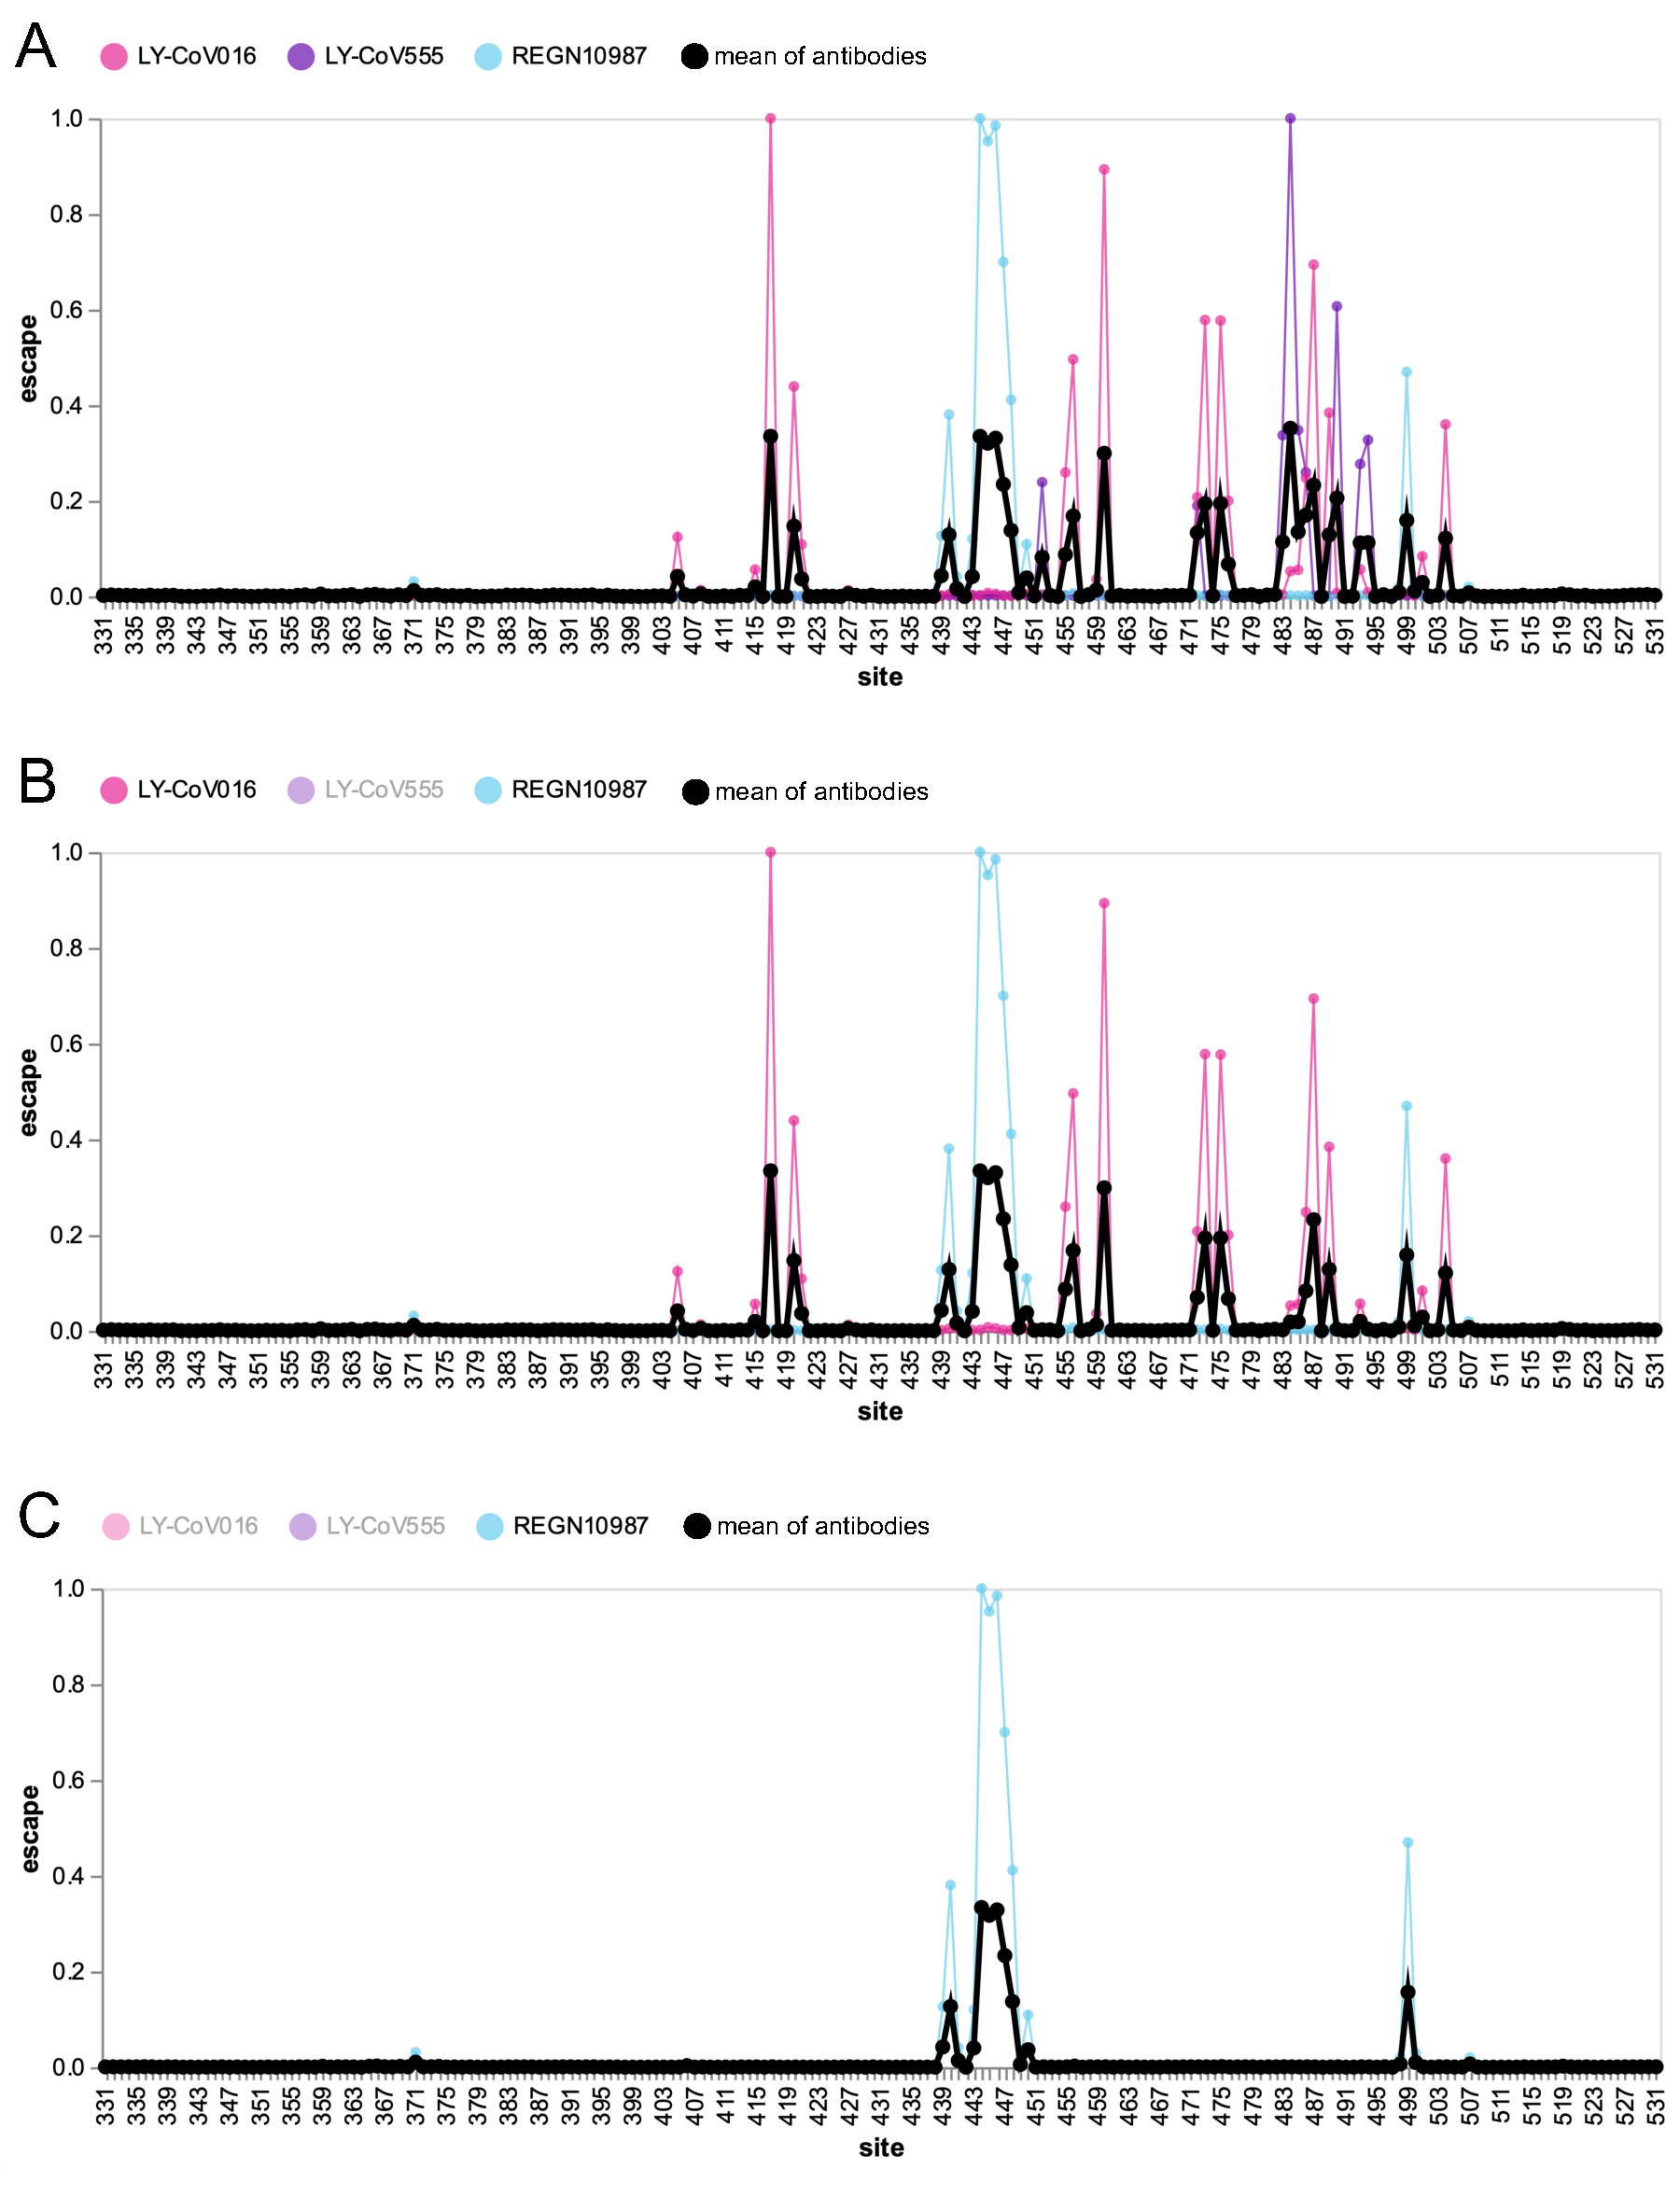
\includegraphics[width=0.71\textwidth]{figures/mini_example/mini_example.pdf} 

\caption{
Escape map for a hypothetical polyclonal mix consisting of an equipotent mixture of three monoclonal antibodies targeting distinct epitopes on the SARS-CoV-2 RBD.
(A) Experimentally measured escape maps for three antibodies, and the mean of these maps (thick black line).
Each point on the x-axis represents a site in the RBD, and the y-axis represents the total measured escape by all mutations at that site scaled so the maximum for each antibody is one.
(B) Escape map if the contribution of antibody LY-CoV555 is ablated.
(C) Escape map if the contributions of antibodies LY-CoV555 and LY-CoV016 are ablated.
An interactive version of this figure is at \url{https://jbloomlab.github.io/SARS2_RBD_Ab_escape_maps/mini-example-escape-calc/}.}
\label{fig:mini_example}
\end{SCfigure*}

\section{Discussion}


{\small

\section{Methods}
\subsection{Code and data availability}

\section{Acknowledgments}
{\color{red} GISAID}
JDB is an Investigator of the Howard Hughes Medical Institute.

\section{Competing interests}
JDB consults for Moderna and Flagship Labs 77, and is an inventor on a Fred Hutch licensed patents related to deep mutational scanning of viral proteins.

}

\bibliography{references}

\end{document}
